\newcommand{\figuraProcesoPolitropico}{%
\begin{figure}[H]
    \centering
    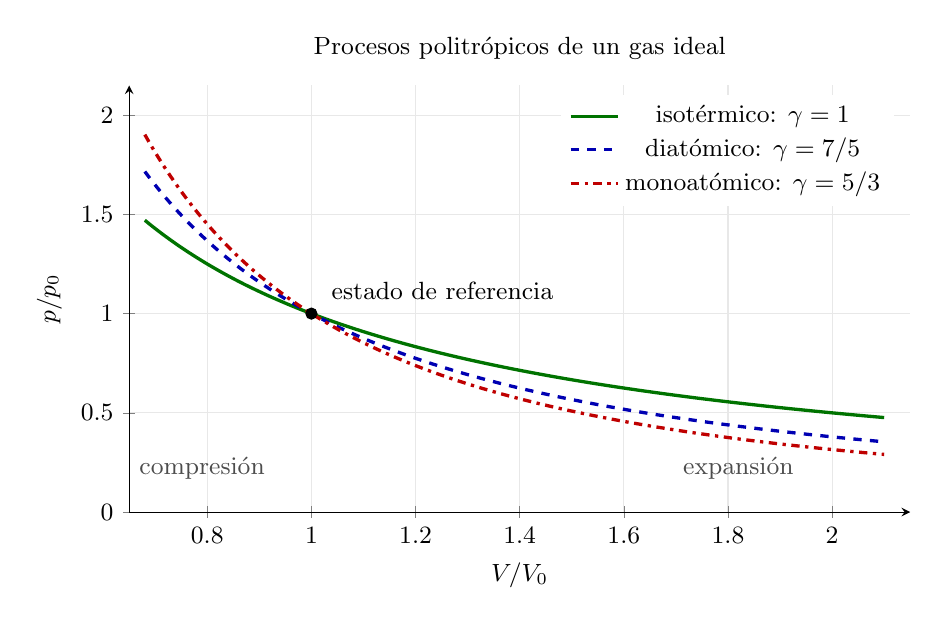
\begin{tikzpicture}[font=\small]
        \begin{axis}[
            width=11.5cm,
            height=7.0cm,
            xmin=0.65,xmax=2.15,
            ymin=0,ymax=2.15,
            axis lines=left,
            xlabel={$V/V_0$},
            ylabel={$p/p_0$},
            title={Procesos politrópicos de un gas ideal},
            grid=major,
            grid style={gray!18},
            samples=180,
            legend style={draw=none,fill=white,at={(0.98,0.98)},anchor=north east}]

            \addplot[very thick,green!45!black,domain=0.68:2.10]
                {x^(-1)};
            \addlegendentry{isotérmico: $\gamma=1$}

            \addplot[very thick,blue!70!black,dashed,domain=0.68:2.10]
                {x^(-1.4)};
            \addlegendentry{diatómico: $\gamma=7/5$}

            \addplot[very thick,red!75!black,dash dot,domain=0.68:2.10]
                {x^(-1.666667)};
            \addlegendentry{monoatómico: $\gamma=5/3$}

            \addplot[only marks,mark=*,mark size=2pt,black]
                coordinates {(1,1)};
            \node[anchor=south west] at (axis cs:1.02,1.02)
                {estado de referencia};

            \node[text=black!70] at (axis cs:0.79,0.22) {compresión};
            \node[text=black!70] at (axis cs:1.82,0.22) {expansión};
        \end{axis}
    \end{tikzpicture}
    \caption{Curvas presión--volumen normalizadas para distintos índices
    politrópicos. Durante una compresión, la presión aumenta más rápidamente
    cuanto mayor es $\gamma$.}
    \label{fig:proceso-politropico}
\end{figure}%
}